\chapter{Frontend}
    Questa parte di applicazione si occupa della visualizzazione dei test.
    Inoltre rende disponibile un'interfaccia per sostituire e committare i test.
    Pu\'o anche essere integrato con un tool esterno per consultare le differenze tra i test.
    \begin{figure}
        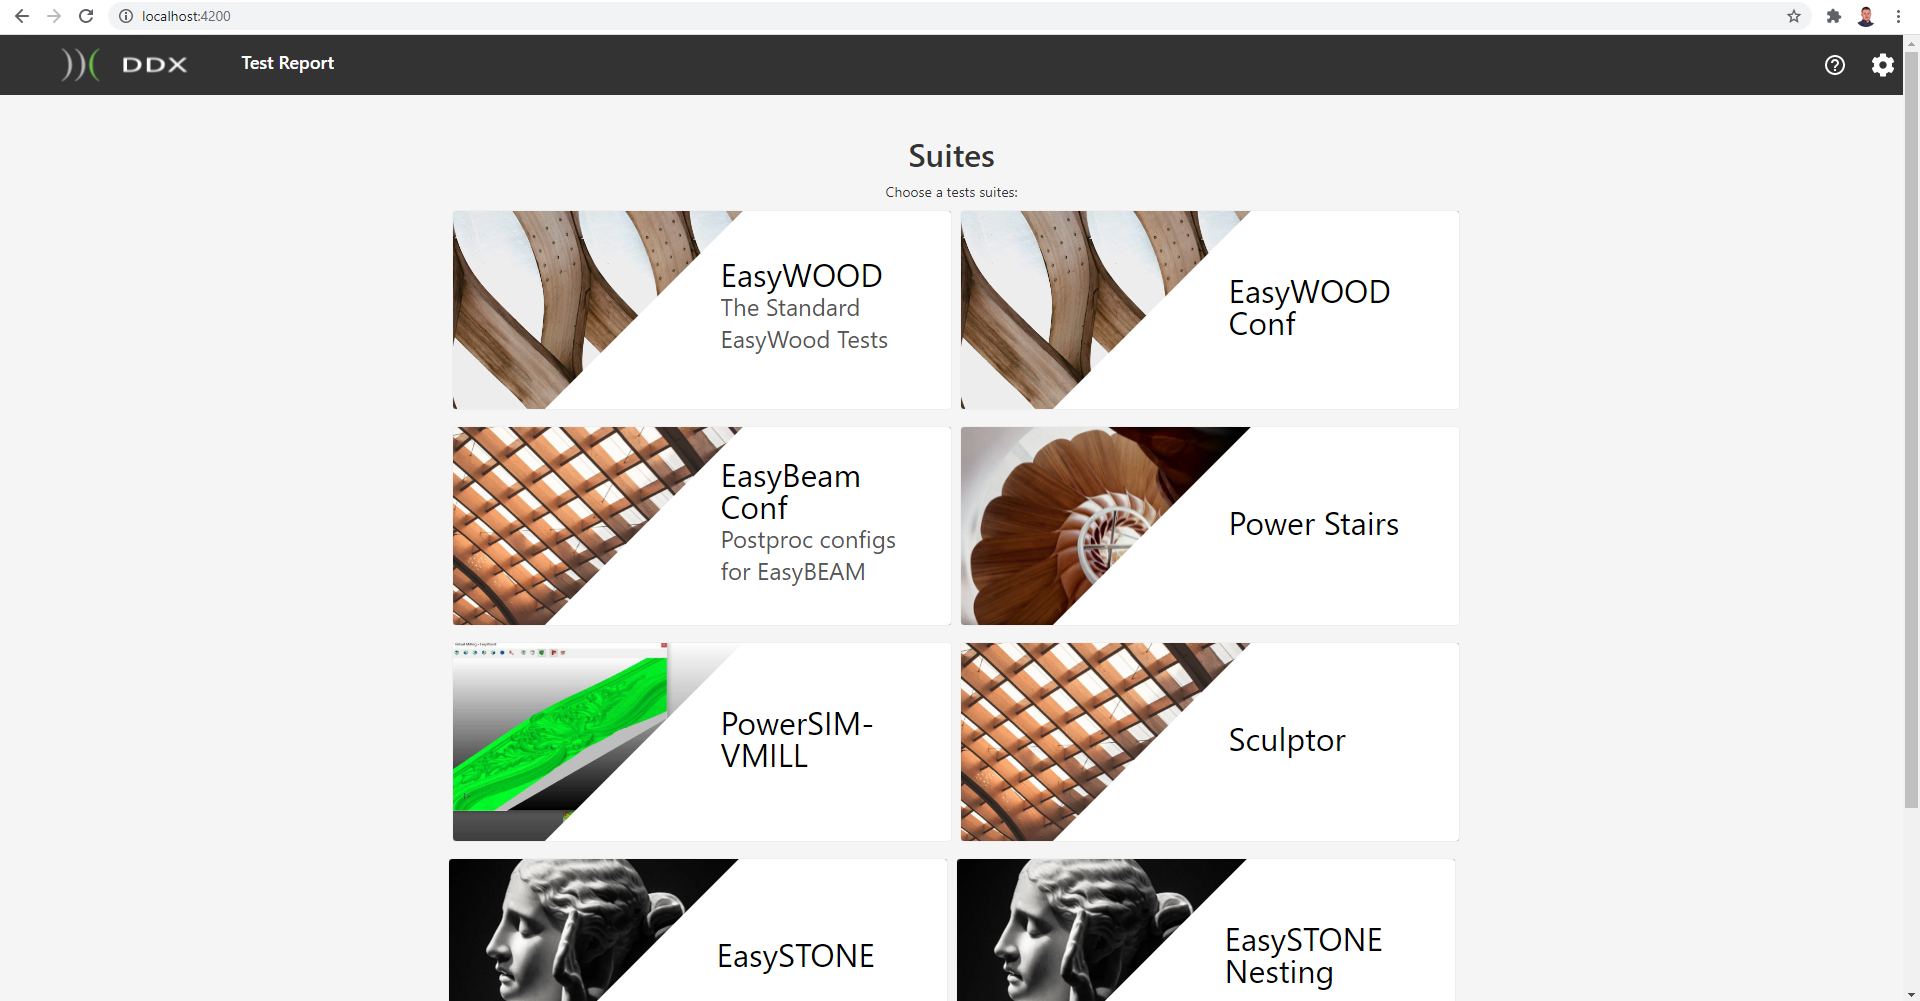
\includegraphics{images/homepage.png}
        \caption{La pagina di home dell'interfaccia web attraverso la quale \'e possibile scegliere quale test suite consultare.}
    \end{figure}
    \section{Angular}
        Angular \'e un framework web che consente di creare applicazioni dinamiche e reattive.    
        Questo framework consente di sviluppare SPA (Single Page application)
        TODO: Spiegare cosa \'e Angular e cosa \'e una single page applicazition SPA
        \subsection{Scelta dell'utilizzo}
            \'E stato scelto di usare Angular, perchè è un framework stabile supportato da Google
            e \'e già stato usato precedentemente per lo sviluppo di altri applicativi.
            
            La struttura a componenti, favorisce il riuso del codice perciò è stato possibile integrare
            nello sviluppo componenti già sviluppati da altri, che forniscono comportamenti base
            come il rendering 3d di un file CAD proprietario.
        
        \subsection{Typescript}
            Un altro motivo per la scelta di Angular è \href{https://www.typescriptlang.org}{Typescript}.
            Typescript è un \textit{superset di javascript} cioè una sua estensione che ingloba tutte le sue feature e ne aggiunge altre.
            La sua peculiarità principale è l'aggiunta di uno step di compilazione che consente di aggiungere una tipizzazione statica.
            Questa tipizzazione consente allo sviluppatore di
            \href{https://www.quora.com/Why-is-type-checking-important-in-programming-languages-and-how-should-one-choose-between-dynamically-and-statically-typed-languages}{ridurre errori banali}.
    \section{Funzionalità}
        La prima responsabilità dell'interfaccia web \'e rendere i test fruibili graficamente.
        Ogni test \'e rappresentato da una card che contiene una lista di references con un indicatore grafico del loro stato.
        \subsection{visualizzazione dei test}        
            Uno scopo del report \'e rendere pi\'u facile individuare i test in base al loro stato.
            \'E perci\'o possibile filtrare i test in base al loro stato e rendere visualizzabili solo quelli con almeno un reference in errore.
            Si pu\'o anche applicare il filtro a un ulteriore livello di profondit\'a e nascondendo le reference corrette all'interno di un test.
            \begin{figure}
                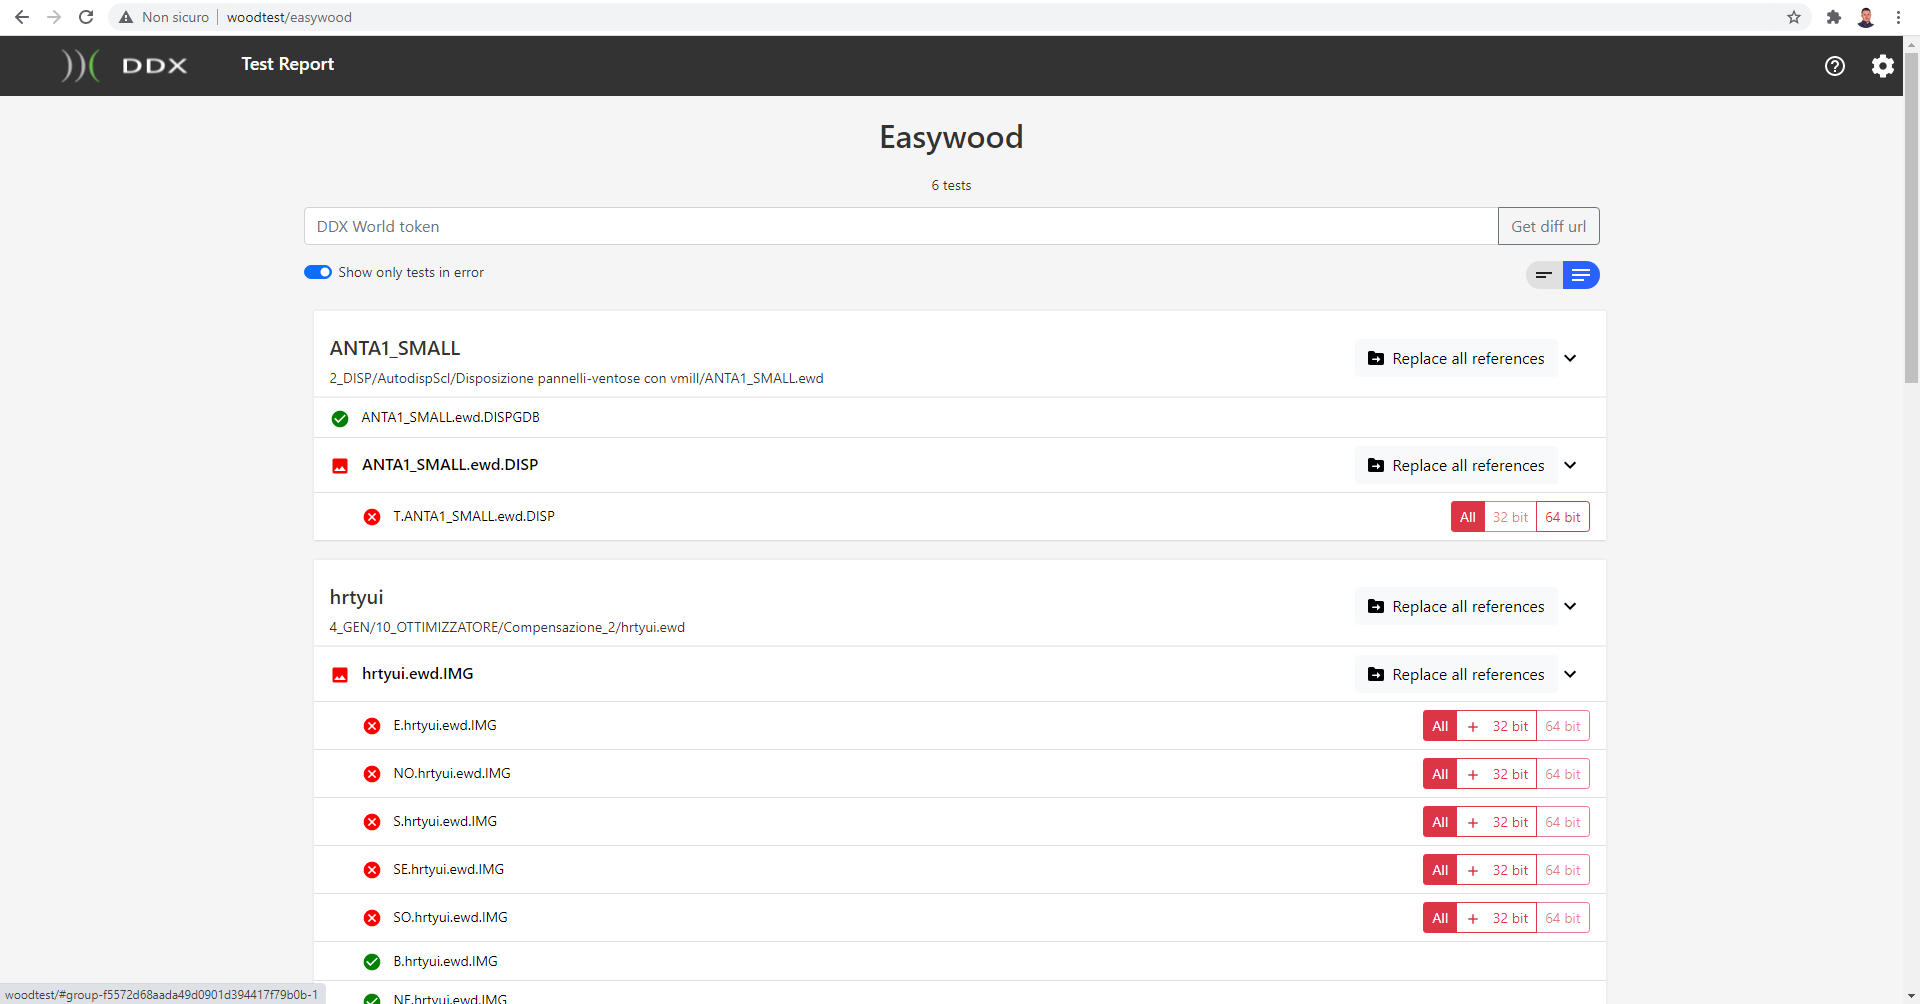
\includegraphics{images/page.png}
                \caption{Un esempio di visualizzazione di test}
            \end{figure}
            \\
            Un ulteriore modo per togliere un test dalla vista \'e l'operazione di \textit{collapse}, essa consente di nascondere tutte le reference lasciando solamente il nome del test.
            Con una specifica pagina di configurazione si pu\'o personalizzare il comportamento del programma in modo che tutti i test vengano collassati all'avvio dell'applicazione.
            
            \begin{figure}
                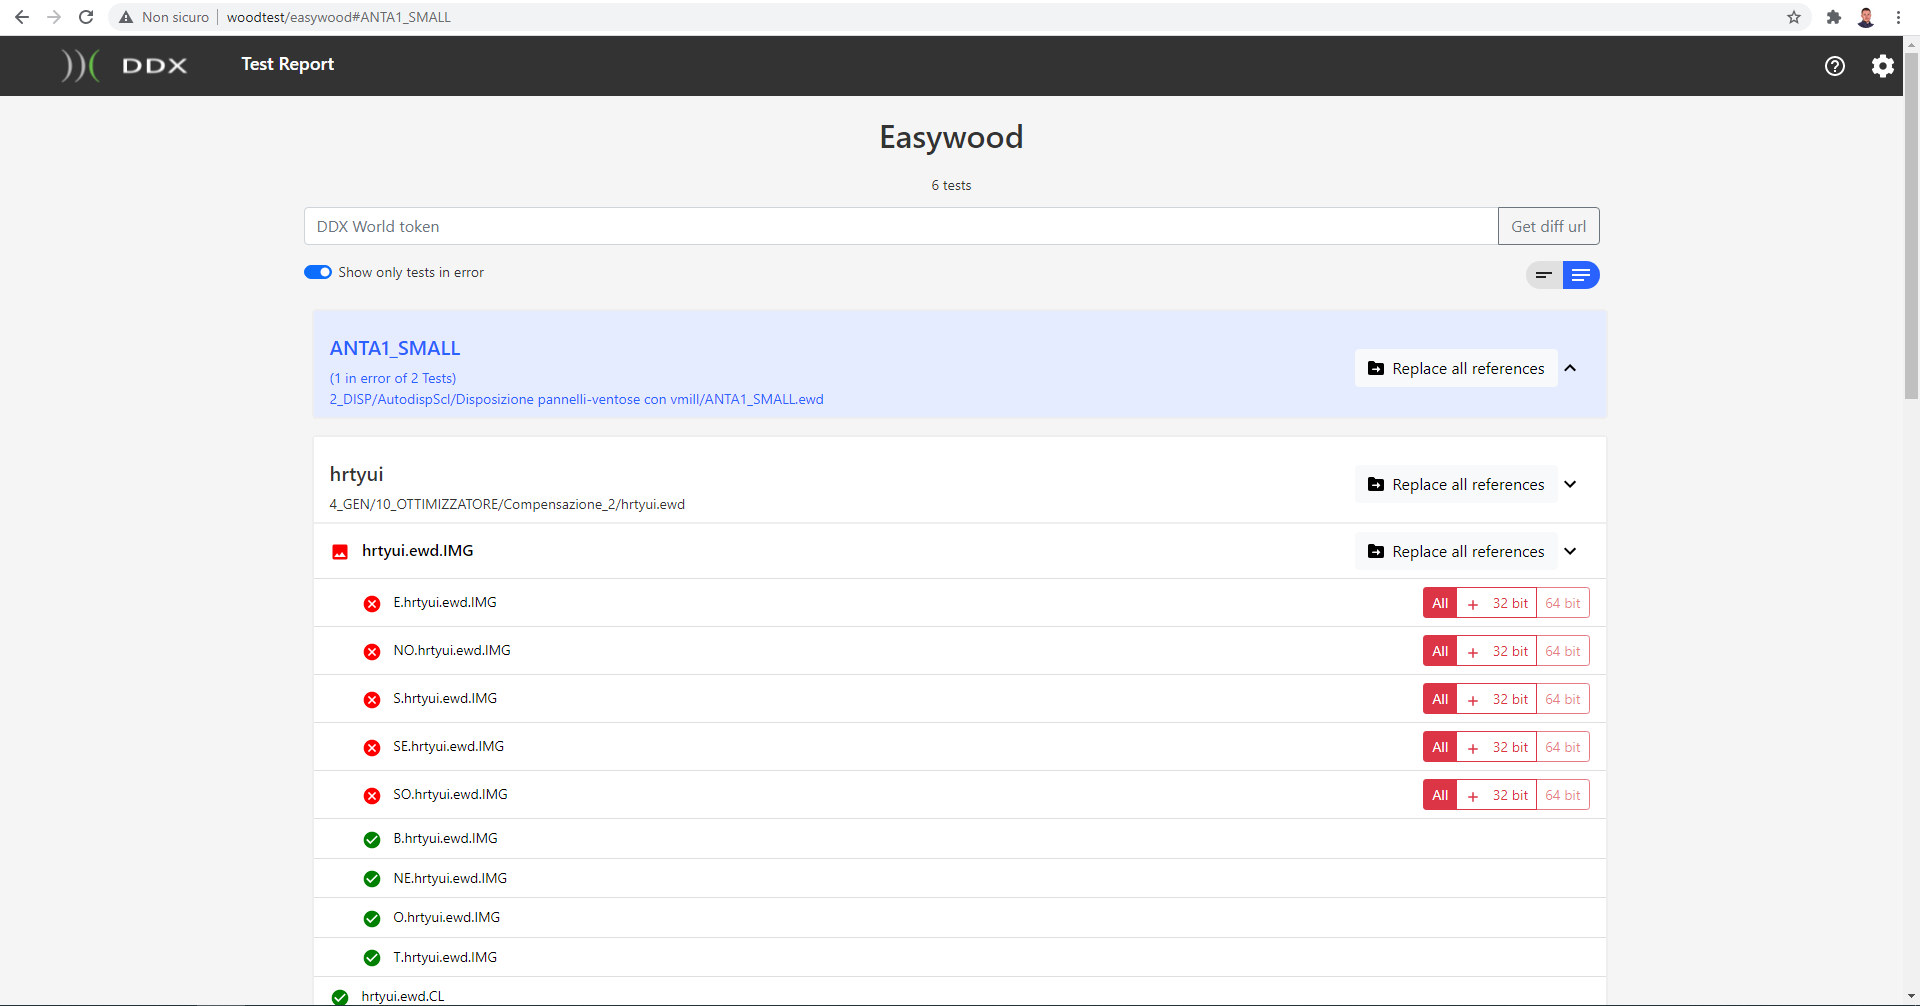
\includegraphics{images/collpapsed.png}
                \caption{Un test in stato \textit{collapsed}}
            \end{figure}
            
            \subsection{Gestione interattiva dei file sovvrascritti}
            L'iter di modifica di un test consiste nel: 
            \begin{itemize}
                \item Confronto di un oracolo con il suo risultato in errore
                \item Aggiunta delle azioni in un area predisposta
                \item Creazione di un commit
            \end{itemize}      
            Il sistema tiene traccia delle azioni effettuate perchè esse non sono effettive e condivise in rete fino a quando non viene creato un commit.
            L'interfaccia web dispone una sezione per salvare le azioni e committarle.
            In un area specifica vengono visualizzate tutte le azioni, che possono essere annullate o definitivamente registrate.
            \subsection{Navigazione}
            \'E  disponibile un metodo di navigazione per aumentare l'usabilità dell'applicazione.
            Durante la navigazione è possibile rendere un test \textit{focussed} e effettuare operazioni (come nasconderlo o metterlo in stage) usando delle scorciatoie da tastiera.\\
            Quando il focus si sposta su un nuovo test la pagina effettua un operazione di scroll per includerlo nella parte visibile della pagina.
            Si puo spostare il focus della navigazione sul prossimo elemento o su quello precedente usando delle scorciatoie da tastiera.
            Lo stato della navigazione viene descritto nell'URL, scrivendo il nome dell'elemento in focus nella sezione denominata \textit{fragment}.\\
            Se la pagina viene richiesta con un fragment già impostato, in fase di rendering dei tests viene posto il focus automaticamente sul test con quel nome (in questo modo sar\'a visualizzabile gi\'a al caricamento della pagina).\\
            Nella filosofia web questo rende condivisibile una risorsa primaria dell'applicazione usando un URL.
            
            \begin{figure}
                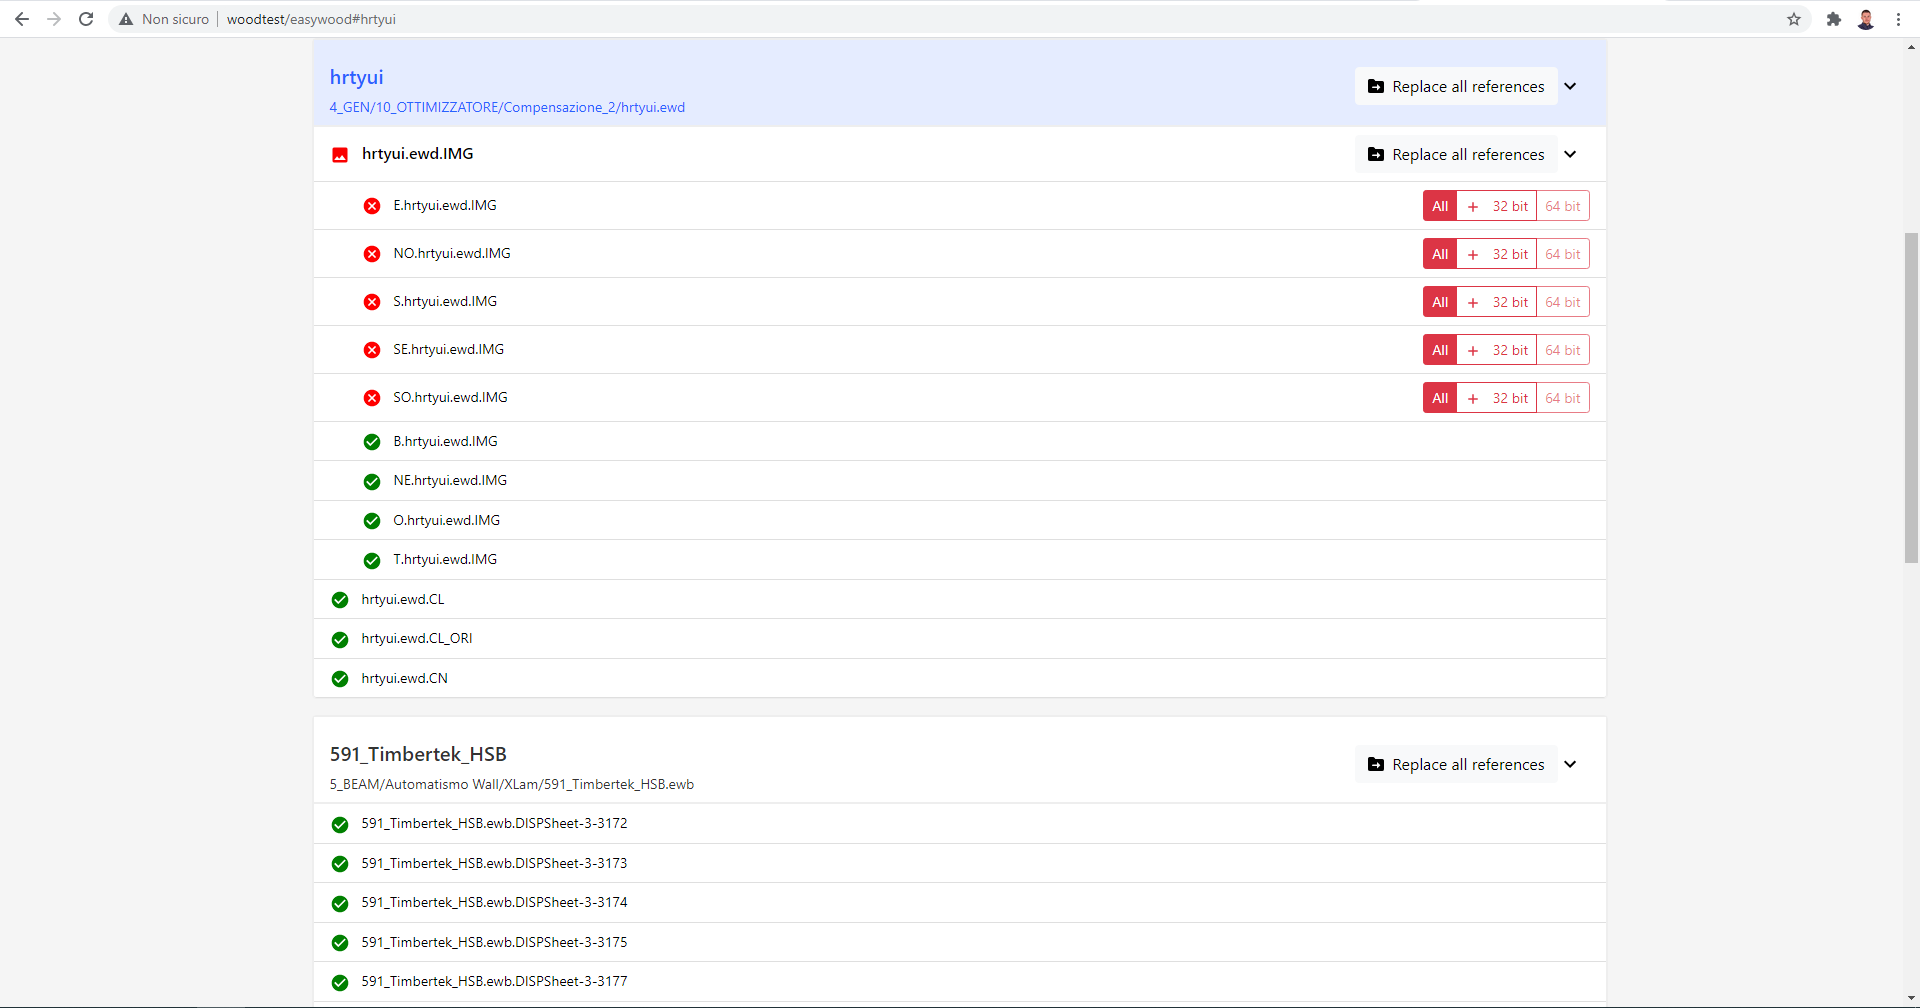
\includegraphics{images/active.png}
                \caption{Un test in stato di focus. La sua scheda relativa viene evidenziata e l'url della pagina viene modificato includendo il nome della risorsa.}
            \end{figure}
            \section{Interazione con gli altri tool aziendali}
            La consultazione delle differenze viene delegata a un tool aziendale già sviluppato in precedenza, denominato \textit{Differ}.
            Anch'esso \'e un tool web quindi questa integrazione avviene  costruendo un URI per navigare nella pagina successiva.
            Il Differ \'e integrato a sua volta con il processo di lancio dei test, e una volta terminato salva le differenze dei test per ogni sessione.
            Il report in oggetto produce un interfaccia in tempo reale con lo stato del server mentre il tool per le differenze salva solo il confronto tra i file reference e current alla fine di ogni sessione.
        perci\'o per sincronizzare lo stato tra i due sistemi \'e necessario recuperare l'ultima sessione di test eseguita e, per ogni reference, creare un url che associ il file con la pagina della differenza.